\documentclass[a4paper]{IEEEtran}
\usepackage{graphicx}
\usepackage{amsmath}
\usepackage{amsfonts}
\usepackage[utf8]{inputenc}
\usepackage{array}
\usepackage{amsmath}
\usepackage{xspace}
\usepackage[section]{placeins}

\newenvironment{conditions}
  {\par\vspace{\abovedisplayskip}\noindent\begin{tabular}{>{$}l<{$} @{${}={}$} l}}
  {\end{tabular}\par\vspace{\belowdisplayskip}}

\inputencoding{utf8}
\renewcommand\IEEEkeywordsname{Index Terms}
\newcommand\nth{\textsuperscript{th}\xspace} %\th is taken already

\title{{\normalsize Autonomous Systems} \\
Localization using Extended Kalman Filter and a LRF}
\author{
        \textbf{Group 15}\\
        R\'{u}ben Tadeia (75268)
        \quad
        Manuel Moura (75756)
        \quad
        Pedro Falcão (77063)
        \quad
        Davi Mello (89126) \\
        Instituto Superior T\'{e}cnico}
\date{\today}

\begin{document}
\maketitle
\hbadness=99999  % or any number >=10000

\begin{abstract}
  The goal of this project is to allow a mobile-robot (Pioneer P3-DX) to localize himself conditioned to the use of Extended Kalman Filter and a Laser Range Finder. The Laser Range Finder will detect the distances to nearby objects (scan the environment) allowing us to acquire a map and then to estimate the localization of the robot pose in that map. 
It's known that the Kalman Filter (KF) is based on a method of
linear Gaussian systems and can be used as a localization method in real systems. Although since some systems are not linear, we need to go a bit further and use the Extended Kalman Filter (EKF) that applies linearizations on non-linear equations. In short, the EKF used is an approximation to the original Kalman Filter. This method gave us the good results, meaning we had small error variation.

\end{abstract}

\begin{IEEEkeywords}
  Localization, Extended Kalman Filter, Laser Range Finder, Mapping, Mobile-Robot
\end{IEEEkeywords}

\section{Introduction}
\label{sec:introduction}

The problem we had to deal with involved a recurring issue in everyday's life: the localization problem. Whether they are smart-phones, our computers or even mobile robots all of them have a method of self-localization, usually by triangulation (GPS). It is therefore a key topic today. \par
Our project consists of locating a mobile robot (Pioneer P3-DX). To accomplish this task we used the Extended Kalman Filter (EKF) with the help of a Laser Range Finder that scans the environment and allows us to acquire a map. The communication platform between the algorithm and the robot is the ROS, which is not only the basis implementation of all parts to a good functioning of the program, but also allows the integration of new packages developed by the user.\par

So as said before we have a global map for the robot. This map is uploaded as an jpeg image and with the help of the laser range finder we identify all of its boundaries, walls, into line segments, with the
occupancy grids method, that divides the environment in cells. In other words, we match a position of the pixel of the image to a distance travelled by the robot. After, we use a method called Least Squares to match a line between the obtained points.\par
The Extended Kalman Filter provides optimal estimates for non-linear systems and is composed by 2 steps the Prediction Step and the Update Step. The EKF helps us find the main objective that is to correct the pose of the robot by subtracting the parameters of matching lines from local and global maps. We have a global map (the uploaded one) and the one that the robot "sees" called the local map, composed by information of the Odometry and the Laser.

The remainder of the paper is organized as follows. In
Section~\ref{sec:methods-algorithms}, we give a brief explanation of the methods used and ROS packages and algorithms used.
Section~\ref{sec:implementation}, divided in sections, describes how the implemented localization algorithm works \textbf{e.g.}, navigation, mapping and task coordination. In Section~\ref{sec:experimental-results} we show the most relevant results to illustrate the merits. Finally, we state our conclusions and lessons learned in Section~\ref{sec:conclusion}. 

\section{Methods and Algorithms}
\label{sec:methods-algorithms}
\textbf{Obtaining the Global Map:}\\
In order to obtain the parameters of the lines of global map we transformed the image of the map in a matrix by the pixel color and we created clusters of points for different lines that are on the map. The lines' equation for each line j is:
\begin{equation}
X_{G}*cos(\alpha_{j})+Y_{G}*sin(\alpha_{j})=\rho_{j}
\end{equation}

\begin{figure}[htp]
  \centering
  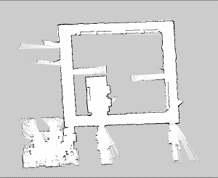
\includegraphics[width=0.9\columnwidth]{./map3}
  \caption{Global Map}
  \label{fig:Global Map}
\end{figure}

\textbf{Obtaining the Local Map:}\\
When the robot moves a new scan of Laser Range Finder is performed and the local map is constructed which consists in a set of line segments described by the equation for each line i is :
\begin{equation}
X_{R}*cos(\psi_{i})+Y_{R}*sin(\psi_{i})=r_{i}
\end{equation}
We use Least Square Method to find this parameters.

\begin{figure}[htp]
  \centering
  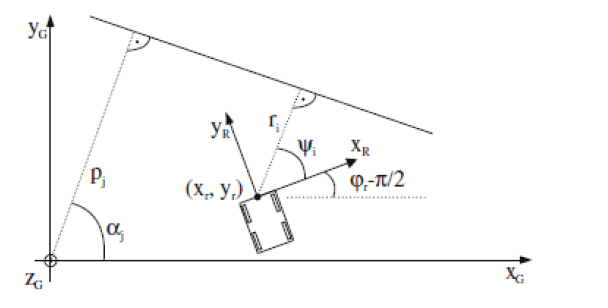
\includegraphics[width=0.9\columnwidth]{./GOBALANDLOCALMAP}
  \caption{Global and Local Map Coordinates.}
  \label{fig:Global and Local Map Coordinates}
\end{figure}

\textbf{Lines Segments Extraction:}\\
For each cycle of data received from de LRF we get a set of distances d between the laser and the obstacle for a set of angles between -90º to 90º.
The data collected by the LRF was first converted into Cartesian coordinates and stored in an array according to the equations:
\begin{equation}
x_{i}=d_{i}*sin(-\theta_{i})
\end{equation}
\begin{equation}
y_{i}=d_{i}*cos(\theta_{i})
\end{equation}
We want to cluster points so we need to analyze if the distance between two consecutive points
is bellow a threshold and if the difference between the angle of those two points and the angle of the line formed by the cluster is bellow a threshold. If this two conditions are verified the point is clustered. If not, the point is excluded from the cluster and the cluster is finalized. 

\textbf{Least Square Method:}\\
We use this method to get $\psi$ and r. 
If a cluster belongs to a vertical line we will not be able to apply this method since the value of the slope will be infinite, so we calculate the approximated value of the scope using the first and the last points of the cluster. If the slope is bigger than 1 we need to apply a rotation of -90º to all points. In the end of the method we need to apply a rotation of 90º to $\psi$ to obtain the correct line parameters.
We use the following equations:
\begin{equation}
\label{eq:U}
\resizebox{1.0\hsize}{!}{ \begin{array}[t]{cc} \hat{\theta}=[\hat{m}_l,\hat{b}_l]^T=(\textbf{U}^T \textbf{U})^{-1} \textbf{U}^T \textbf{y}, \quad 
\textbf{U}=\begin{bmatrix}
       \textbf{x}(1) & \cdots & \textbf{x}(n) \\
       1 & \cdots & 1 \\
  \end{bmatrix}^T,\\
\\
\textbf{y}=[\textbf{y}(1),\cdots,\textbf{y}(n)]^T,
\end{array}
}
\end{equation}
%
where $n$ is the number of points of the cluster; $\hat{m}_l$ and $\hat{b}_l$ correspond to the line parameters of the line equation in the form $y=m_lx+b_l$. Now we obtain $\psi$ and $\textit{r}$ with

\begin{equation}
\label{eq:r}
r(\hat{m}_l,\hat{b}_l) = \frac{\hat{b}_l}{\sqrt{\hat{m}_l^2 +1}}sign(\hat{b}_l),
\end{equation}
\begin{equation}
\label{eq:psi}
\psi (\hat{m}_l) = \arctan2 \left(\frac{sign(\hat{b}_l)}{\sqrt{\hat{m}_l^2 +1}},\frac{- \hat{m}_l}{\sqrt{\hat{m}_l^2 +1}}sign(\hat{b}_l)\right),
\end{equation}


\textbf{Estimation of Line Parameters covariances:}\\
For the update in EKF we need to compute the covariance matrix $R_{i}$ that is composed by the variance of the line parameters, $r_{i}$ and $\psi_{i}$, and the covariances between them.
\begin{equation}
\label{eq:Ce}
\textbf{Ce}=var(\textbf{y}(j))(\textbf{U}^T \textbf{U})^{-1}=\begin{bmatrix}
       var(\hat{m}_l) & cov(\hat{m}_l,\hat{b}_l) \\
       cov(\hat{m}_l,\hat{b}_l) & var(\hat{b}_l) \\
  \end{bmatrix},
\end{equation}
\begin{equation}
 \label{eq:vary}
var(\textbf{y}(j))=\frac{\sum_{j=1}^{n} (\textbf{y}(j)-\hat{\textbf{y}}(j))^2}{n-1}, \hat{\textbf{y}}(j)=\hat{m}_l \cdot \textbf{x}(j)+\hat{b}_l
\end{equation}

where $var(\textbf{y}(i))$ is the vertical error variance of the line-segment points (\textbf{x}(j),\textbf{y}(j)) (\textit{j}=1,...,\textit{n}) according to the estimated line with the parameters $\hat{m}_l$ and $\hat{b}_l$. We can now calculate the variances and covariances between the parameters \textit{r} and $\psi$ as follows.
\begin{equation}
\label{eq:varparameters}
\begin{aligned}
var(\psi) & = K_{\psi }^2 var(\hat{m}_l),\\
var(r) & = K_{r m}^2 var(\hat{m}_l)+K_{r b}^2 var(\hat{b}_l)+2 K_{r m}K_{r b} \cdot cov(\hat{m}_l,\hat{b}_l),\\
cov(r,\psi) & = K_{r m} K_{\psi m} var(\hat{m}_l) + K_{r b} K_{\psi m} \cdot cov(\hat{m}_l,\hat{b}_l), \\
cov(\psi ,r) & = cov(r, \psi),
\end{aligned}
\end{equation}
where
\begin{equation}
\label{eq:ks}
\resizebox{1.0\hsize}{!}{ \begin{array}[t]{lcl} K_{r m}=\frac{-\hat{b}_l\hat{m}_l}{\sqrt[]{\hat{m}_l^2+1}(\hat{m}_l^2+1)}sign(\hat{b}_l), \quad K_{r b}=\frac{sign(\hat{b}_l)}{\sqrt[]{\hat{m}_l^2+1}}, \quad K_{\psi m}=\frac{1}{\hat{b}_l^2+1}. 
\end{array}
}
\end{equation}

\textbf{Local and Global Map Matching:}\\




\section{Implementation}
\label{sec:implementation}

\textbf{State Definition:}\\
Our state is defined by a vector with the position, the angle, the linear and the angular velocities.
Because of that we need to take in consideration one issue 
The initial state is defined with the first values of our measurements and we put them in a measurements vector that we called X.\\

\[
x
=
\begin{bmatrix}
    x       \\
    y    \\
    \Psi      \\
    v      \\
    \dot{\Psi}       
\end{bmatrix}
\]\par
where:
\begin{conditions}
 x     &  Position X \\
 y     &  Position Y \\
 \Psi     &  Heading \\
 v     &  Velocity \\   
 \dot{\Psi} &  Yaw Rate
\end{conditions}


\textbf{Prediction Step (Time update):}

The dynamic model represents the behaviour of the robot over time. The behaviour is described as a set of states that occur in sequence. We implement a dynamic function G with the equations below to calculate how the state is evolving from step to step.

\[
G
=
\begin{bmatrix}
    x + {\frac{v}{\dot{\Psi}}}(-sin(\Psi)+sin(T\dot{\Psi} +\Psi))      \\
    y + {\frac{v}{\dot{\Psi}}}(cos(\Psi)-cos(T\dot{\Psi} +\Psi))   \\
    T\dot{\Psi} +\Psi      \\
    v      \\
    \dot{\Psi}       
\end{bmatrix}
\]
\\

The model is non-linear so we have to linearize it as the extended Kalman filter is only efficient to linear models. We implement the Jacobian of the dynamic matrix $J^{}_A$ regarding the state vector x by calculating the entries of the matrix and then inserting them into it.

The disturbances of the states are described in a process noise covariance matrix Q.
Finally, we project the error covariance ahead P.

\begin{equation}
P_{k+1}=J^{}_A * P_k * {J^{}_A}^T + Q
\end{equation}
\\

\textbf{Measurement Update (Correction):}\\

So now we have our measurement function H with the laser measured values of the position, orientation, linear and angular velocities.


This function can be used to compute the predicted measurement from the predicted state. We linearize it by calculating the Jacobian of this matrix $J^{}_H$ in order to apply the filter.


The measurement noise covariance R entries are defined by attributing variances to the measurements of the laser range finder.


Then we are set to build our Kalman Gain from the measurement Jacobian matrix, the projected error covariance matrix P and the measurement noise covariance matrix R.

\begin{equation}
K_{k}=P_k{J^{}_H}^T(J^{}_HP_k{J^{}_H}^T + R)^{-1}
\end{equation}
where:
\begin{conditions}
 K_{k}     &  Kalman Gain \\
 P_k     &  Projected error covariance matrix \\   
 {J^{}_H} &  Jacobian of the Measurement function \\
 R     &  Measurement noise covariance matrix
\end{conditions}

We update the estimate of the state by summing the previous state to the Kalman gain times the residual (innovation) that is the difference between time measurements. 

\begin{equation}
x_{k+1}=x_{k}+K_{k}(z_{k}-h(x_{k}))
\end{equation}
where:
\begin{conditions}
 x_{k+1}     &  Current state estimate \\
 x_{k}     &  Previous state estimate \\   
 z_{k}-h(x_{k}) &  Residual
\end{conditions}

Finally, we update the error covariance which tells the Extended Kalman Filter how much to trust the measurements and the predictions.

\begin{equation}
P_{k}=(I-K_{k}{J^{}_H})P_{k}
\end{equation}

We stored all the variables and plot them. As you can see in the next section.
\\

\begin{figure}[t!]
    \centering
    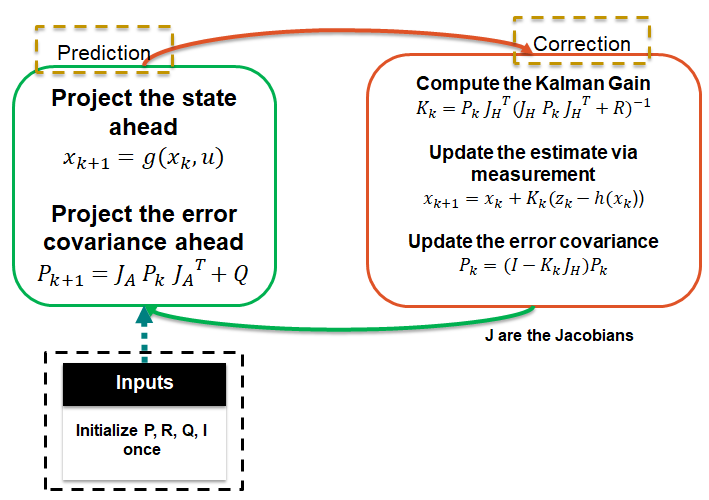
\includegraphics[scale=0.33]{ekf}
    \caption{Extended Kalman Filter diagram}
\end{figure}


%%%%%%%%%%%%%%%%%%%%%%%%%%%%%%%%%%%%%%%%%
%%%%%%%%%%%%%%%%Results%%%%%%%%%%%%%%%%%%
%%%%%%%%%%%%%%%%%%%%%%%%%%%%%%%%%%%%%%%%%
\section{Experimental Results}
\label{sec:experimental-results}

In this section we present the results obtained. Firstly, once all modules have been functioning individually, meaning, that we obtained results as expected.\par
One thing to notice is that since our EKF is velocity based, we had to come up with a solution for a bug with the Laser, because it became sensitive the the angular velocities. These solutions are to first \textbf{ignore values from Laser} when we have quick variances in the distances. For instance, this can happen when an object or person crosses the robot's path. The other solution was to stop reading Laser data when the robot was \textbf{rotation or just changing the orientation}. \par
For the kidnapping solution, we used the Global and local mapping matching method and run it in it parallel. Then we obtained a prediction of $> K \% $, comparing it with the EKF, we get an error of $> \ epsilon \% $. Now we just have to restart the EKF, with the starting position given by the Global and local mapping matching method.\\

Solving the problem of kidnapping by re-calibrating the position of the robot over time.

\begin{figure}[!ht]
  \centering
  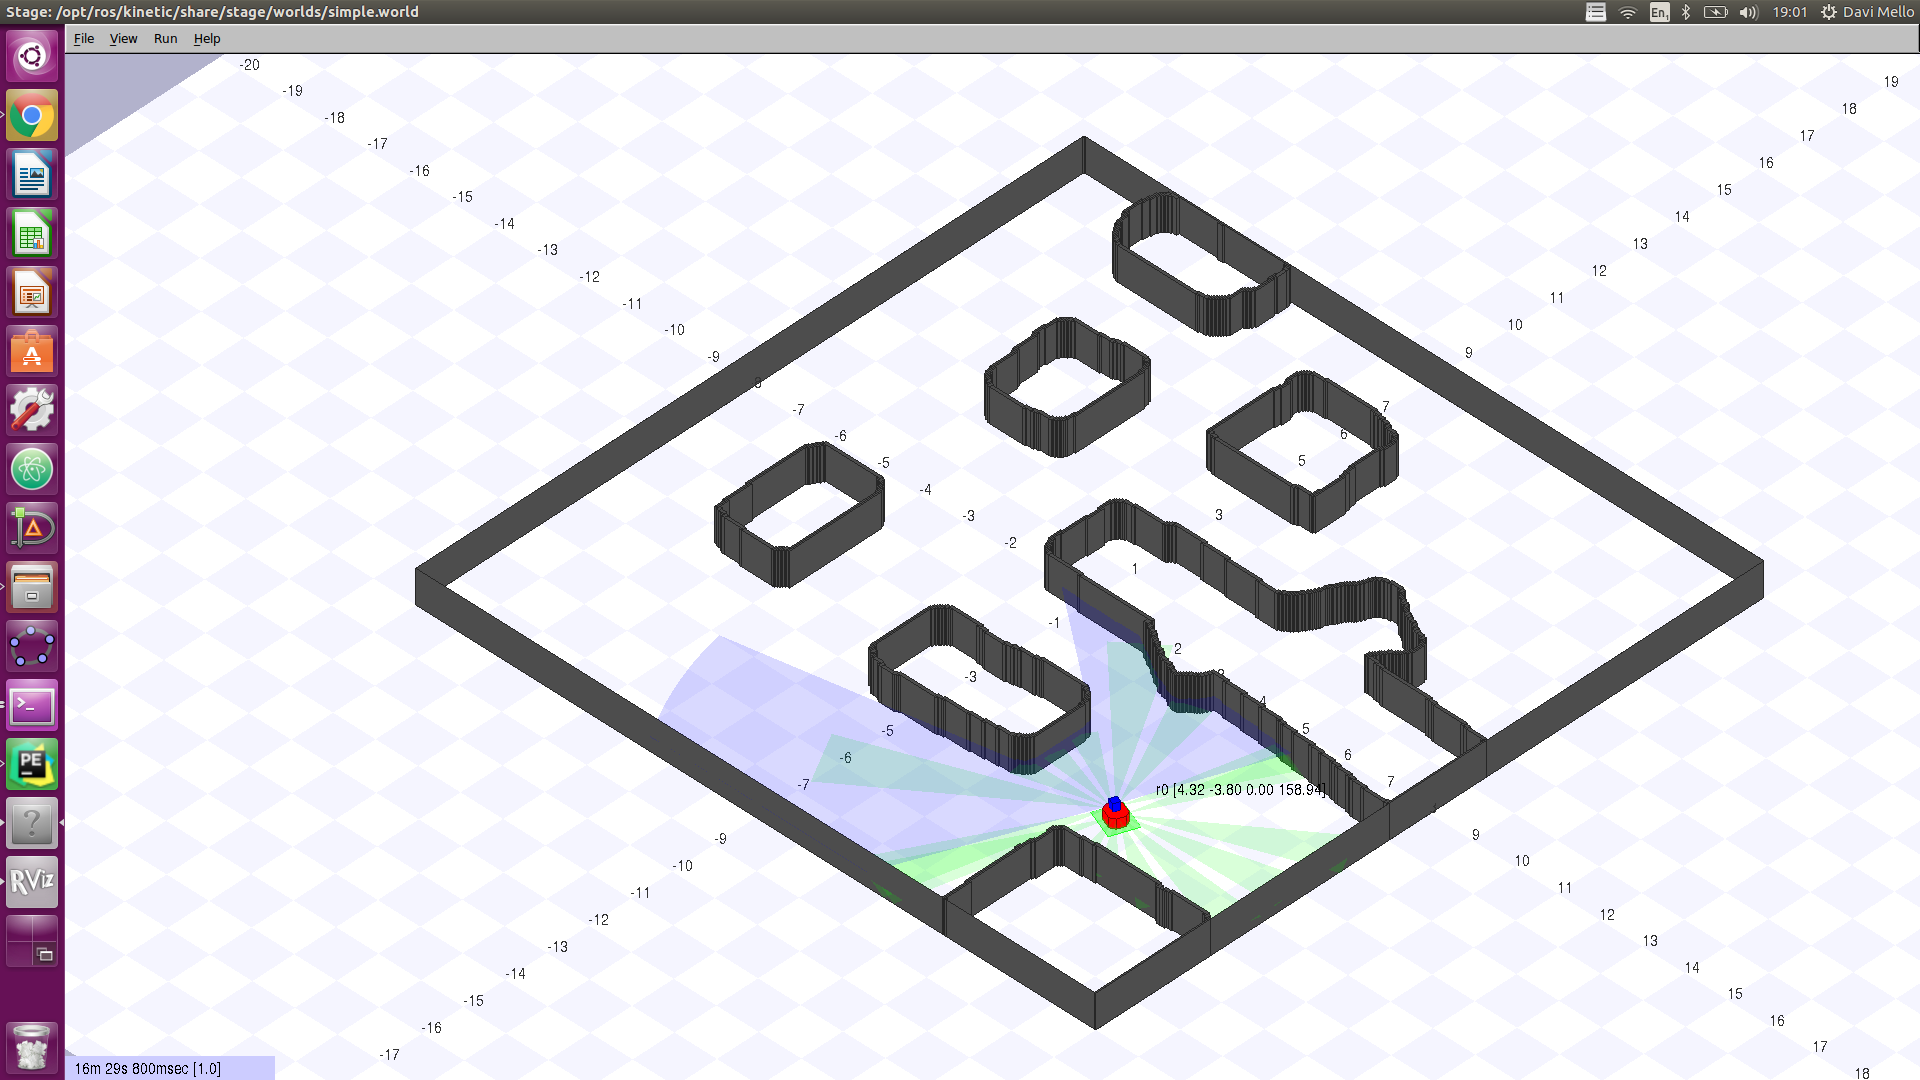
\includegraphics[width=0.8\columnwidth]{./simulation}
  \caption{Testing EKF and LRF in simulation mode}
  \label{fig:simulation}
\end{figure}

\begin{figure}[!ht]
  \centering
  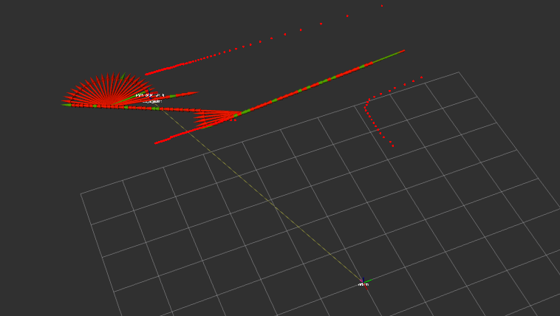
\includegraphics[width=0.8\columnwidth]{./rviz}
  \caption{Testing the EKF in a simulation environment}
  \label{fig:rviz}
\end{figure}

So as we can see from the image above, Figure~\ref{fig:simulation}, we run a simulation using the tele-operation method and observed the result in Figure~\ref{fig:rviz}. In which the red arrows are the robot orientation, the red dots are laser data readings and the green dots are EKF predictions.\\

\begin{figure}[!ht]
  \centering
  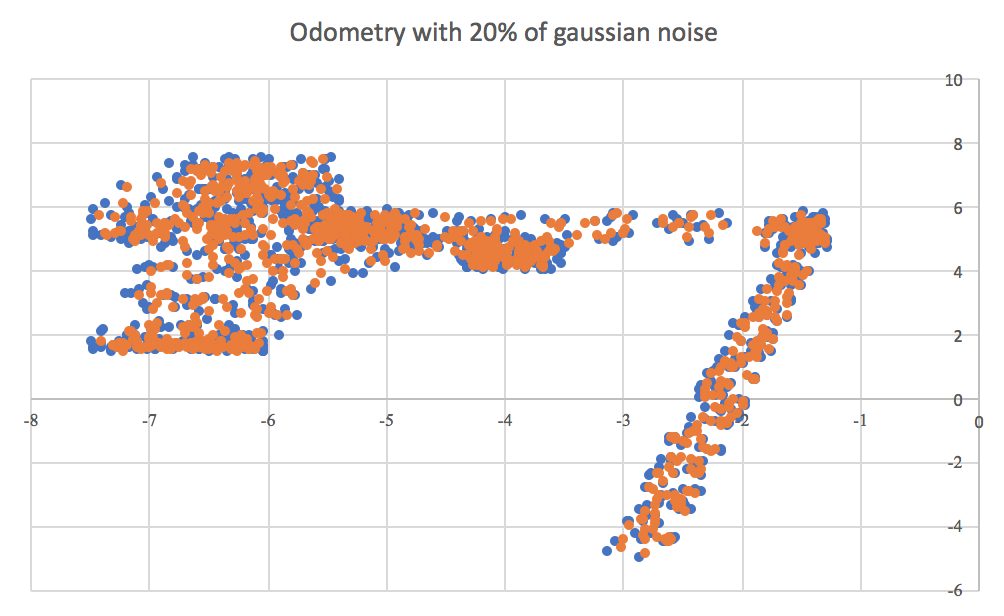
\includegraphics[width=0.8\columnwidth]{./odometry20}
  \caption{Result with an Odometry with 20\% of random noise}
  \label{fig:odometry20}
\end{figure}


\begin{figure}[!ht]
  \centering
  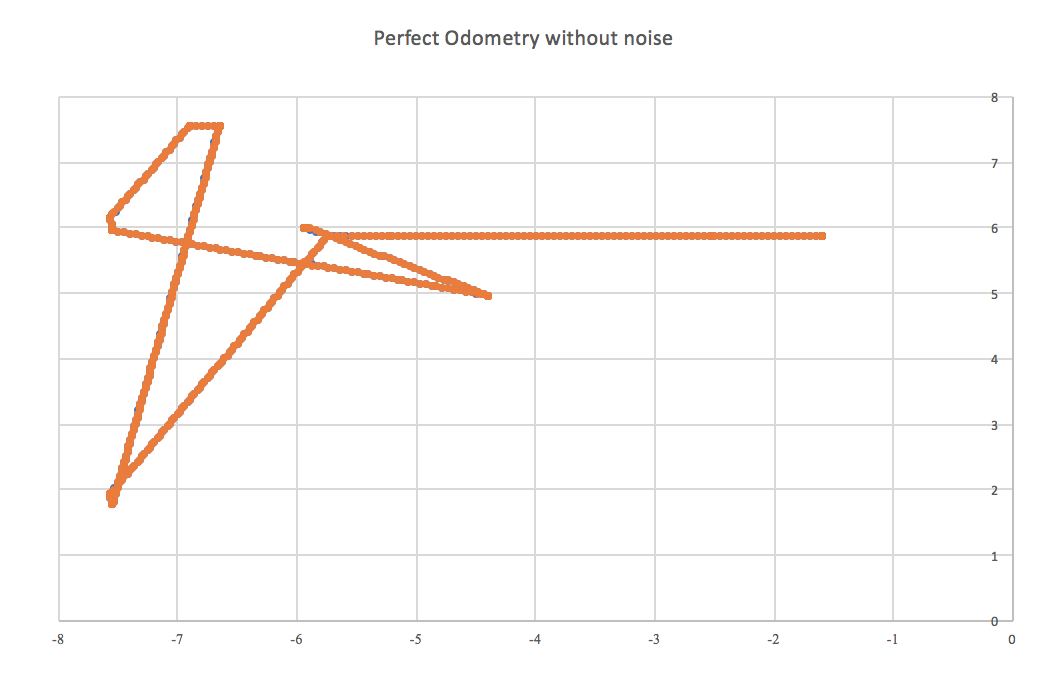
\includegraphics[width=0.8\columnwidth]{./perfectodometry}
  \caption{Result with an Odometry without noise}
  \label{fig:perfectodometry}
\end{figure}

Considering the images above, one thing to have in mind is that the frequency is 10Hz and generated 600 Points, meaning we run it for this image for 1 minute, although the code can run for undetermined time. The first image is Figure~\ref{fig:odometry20} which shows values from Odometry with 20\% random noise,and Figure~\ref{fig:perfectodometry}, without random noise. \par
We results are pretty clear. Without noise the results are very good, and the Extended Kalman Filter values and the Odometry ones are overlapped. Considering the 20\% noise Odometry results, we can see that the algorithm is working acceptably well, although with some discrepancies on some points. 

\begin{figure}[!ht]
  \centering
  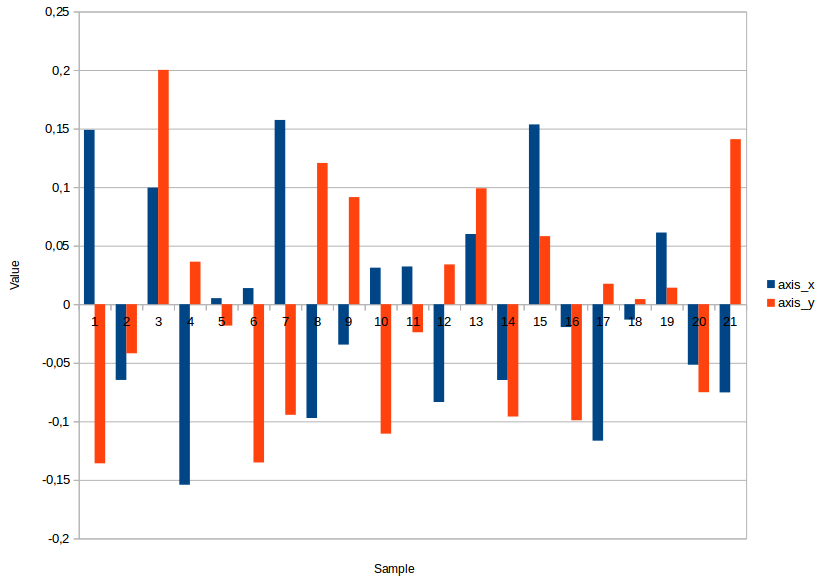
\includegraphics[width=0.8\columnwidth]{./prove}
  \caption{Prove of EKF working (Subtraction of points)}
  \label{fig:prove}
\end{figure}

Finally the Figure~\ref{fig:prove} proves our result on EKF of error in the order of $10^{-3}$. The way we plot this was with some points (fifty) from the perfect Odometry (without noise) and subtracted the values from the predictions resulting from EKF. And the output can be observed.


%%%%%%%%%%%%%%%%%%%%%%%%%%%%%%%%%%%%%%%%%
%%%%%%%%%%%%%%%%%%%%%%%%%%%%%%%%%%%%%%%%%
%%%%%%%%%%%%%%%%%%%%%%%%%%%%%%%%%%%%%%%%%

\section{Conclusions}
\label{sec:conclusion}

In Autonomous Systems, for a mobile robot to function properly, we need to have proper readings and decide upon those to find the best possible action. So it's intended that these readings are as accurate as possible. Here the considered readings were the Laser Range Finder and Odometry ones.
For that reason the EKF algorithm described above, is implemented in order to minimize the errors, for the sake of a more accurate robot localization.
Both the EKF and the Laser data are more accurate than the result from Odometry. That's one of the reasons why the EKF is a "complement" widely used in autonomous systems.
We note that it's important to do the readings as soon as possible so that the whole process can be fluid, in search of the robot determination of its location in real time.
With the work developed, it was possible to understand that it is necessary to minimize all possible
errors, not only because the accuracy of readings is a very crucial factor for good operation but to avoid the propagation of errors that can prove to be disastrous too.\par
In short, since the EKF uses a linearized model, the first thing to do is linearize the kinematic model to perform the prediction step. Then we perform the matching step extracting the parameters from the map of the 5\nth floor the North Tower of Instituto Superior Técnico. From there we had to compare the results from the Laser Range Finder. Finally we go into the update step, that updates robot's position estimation.
It's interesting to note that when using the Harris detection method, in order to achieve the maximum similarity between lines, the extracted points of each line were the first and last ones. This will be later the solution for the kidnapping problem.
In this report, some results were not present \textit{e.g.}, the values obtained for the covariance matrices and better comparisons between the errors obtained with EKF algorithm.\par
Nonetheless these results as well as the matching step from the EKF (consisting in a comparission with the lines between the local and the global map), and a self-explanatory video will be presented in the poster section. Some reasons for things that could had gone better were the group's lack of experience regarding ROS and Python, as a result the group spent more hours learning this basic tools than with the algorithm itself.

\begin{thebibliography}{9}

\bibitem{Slides}
  Pedro Lima,
  \emph{Notas das Aulas Teóricas},
  \texttt{Lisboa - Instituto Superior Técnico},
  2017

\bibitem{EKF}
  Python Implementations
  \emph{of the Kalman Filter},
  \texttt{https://balzer82.github.io/Kalman/}
  
\end{thebibliography}



\end{document}
This is never printed 